\chapter{Análise e Modelação do Sistema}

\section{Site Map}

O Site Map apresenta a estrutura e organização das principais páginas que constituem o sistema GrabATable, permitindo visualizar a hierarquia de navegação e a forma como as diferentes áreas e funcionalidades se encontram interligadas. Este permite também identificar os diferentes perfis de utilizador e as páginas e funcionalidades a que cada perfil terá acesso, proporcionando uma visão global da estrutura e navegação da plataforma.

\begin{figure}[H]
    \centering
    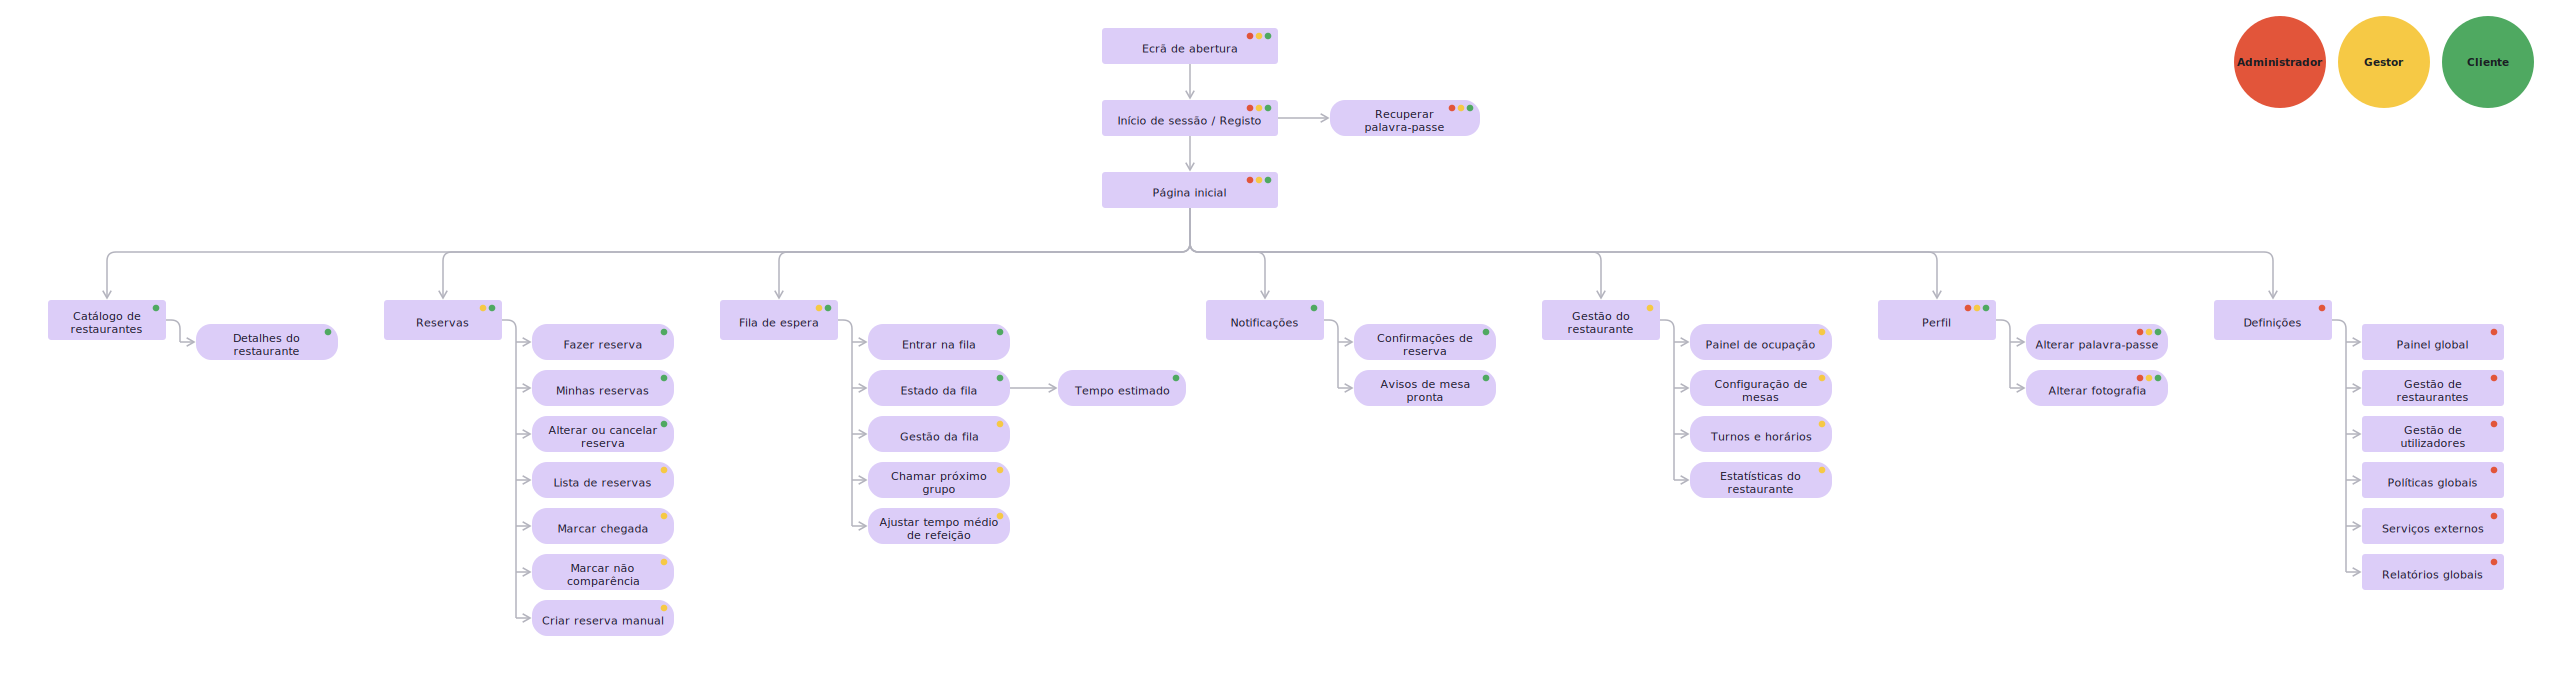
\includegraphics[width=1.0\linewidth]{images/Site_Map.png}
    \caption{Site Map}
    \label{fig:3}
\end{figure}

Todos os perfis partilham o ecrã de abertura, o registo e a página inicial.

\section{Task Model}\label{sec:task-model}

O \textit{Task Model} representa as principais tarefas que podem ser realizadas pelos diferentes perfis de utilizador no sistema GrabATable. Este modelo permite identificar e organizar as ações necessárias para a execução das principais funcionalidades da plataforma, evidenciando a relação entre os utilizadores e as tarefas que estes podem realizar.

\subsection{\textit{Task Model} - Administrador} 

\begin{figure}[H]
    \centering
    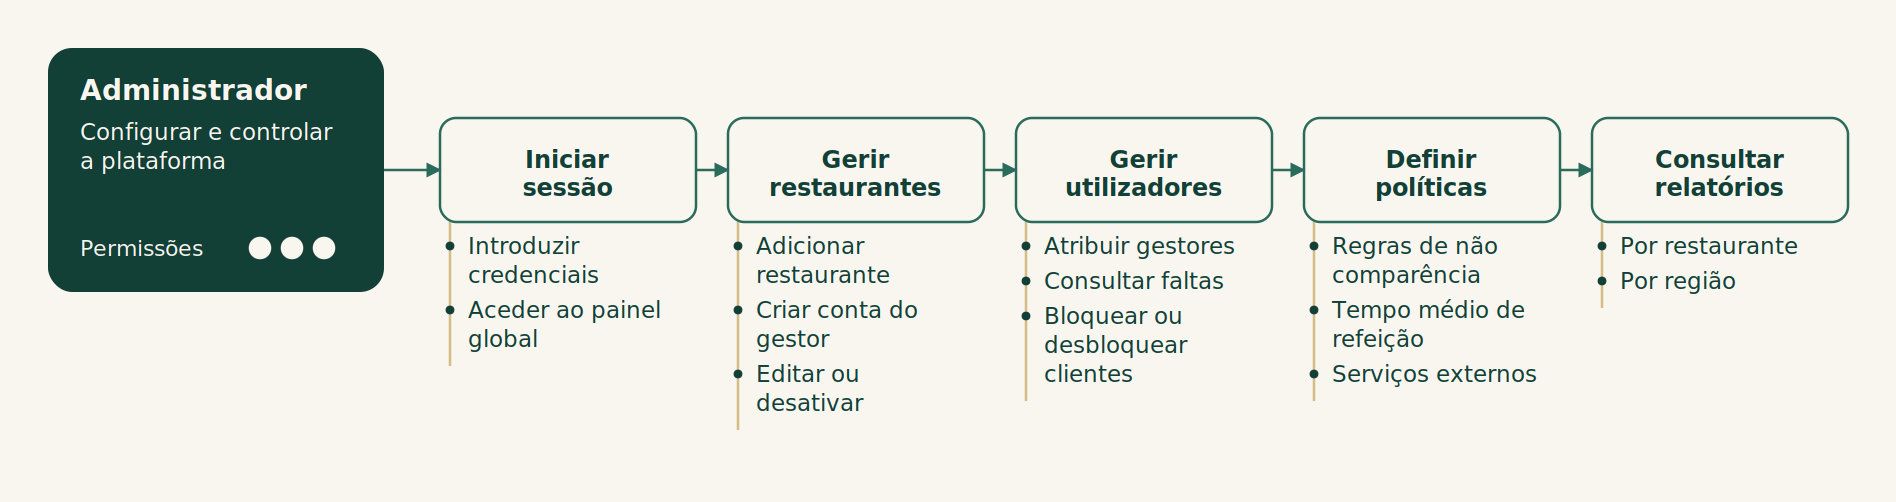
\includegraphics[width=1.0\linewidth]{images/Task_Model_Administrador.png}
    \caption{Task Model - Administrador}
    \label{fig:4}
\end{figure}

\subsubsection{Tarefa principal - Administrador}

Processo para um administrador adicionar um restaurante à plataforma.

\begin{figure}[H]
    \centering
    
\includegraphics[width=1.0\linewidth]{images/Task_Model_1_Administrador_horizontal.png}
    \caption{Tarefa principal - Administrador}
    \label{fig:5}
\end{figure}

\subsection{\textit{Task Model} - Gestor}

\begin{figure}[H]
    \centering
    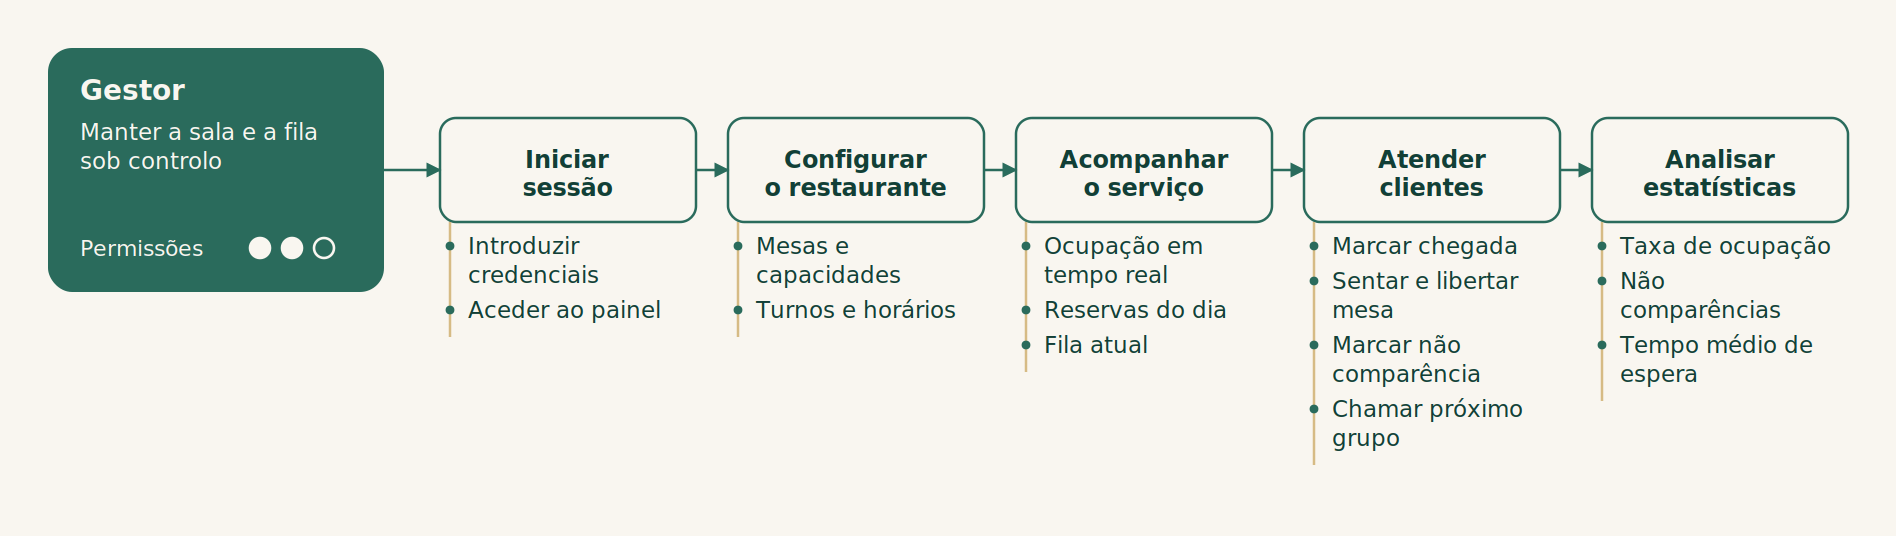
\includegraphics[width=1.0\linewidth]{images/Task_Model_Gestor.png}
    \caption{Task Model - Gestor}
    \label{fig:6}
\end{figure}

\subsubsection{Tarefa principal - Gestor}

Processo para um gestor atender um cliente com reserva.

\begin{figure}[H]
    \centering
    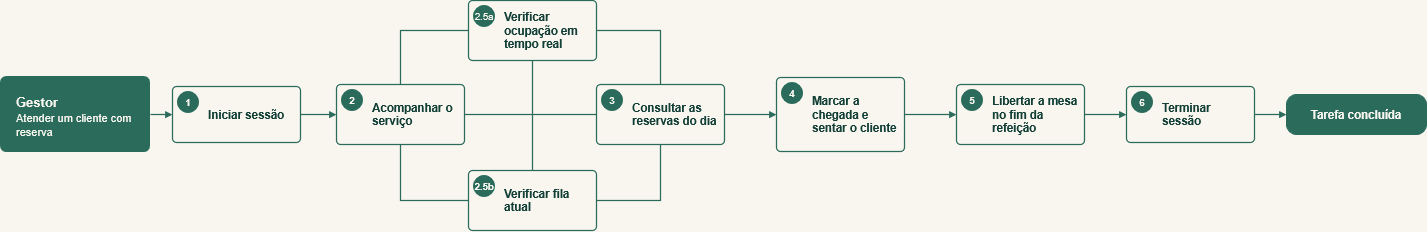
\includegraphics[width=1.0\linewidth]{images/Task_Model_2_Gestor_horizontal.png}
    \caption{Tarefa principal - Gestor}
    \label{fig:7}
\end{figure}

\subsection{\textit{Task Model} - Cliente}

\begin{figure}[H]
    \centering
    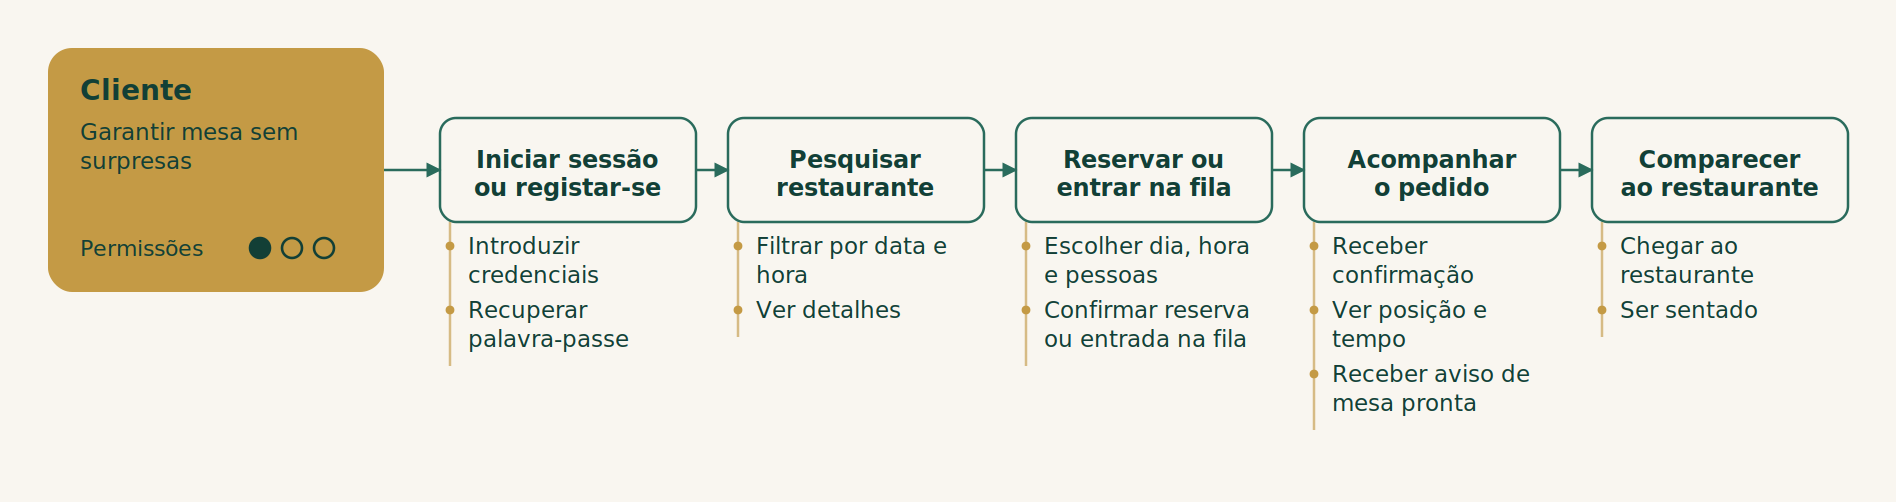
\includegraphics[width=1.0\linewidth]{images/Task_Model_Cliente.png}
    \caption{Task Model - Cliente}
    \label{fig:8}
\end{figure}

\subsubsection{Tarefa principal - Cliente}

Processo para um cliente reservar mesa para refeição.

\begin{figure}[H]
    \centering
    
\includegraphics[width=1.0\linewidth]{images/Task_Model_3_Cliente_horizontal.png}
    \caption{Tarefa principal - Cliente}
    \label{fig:9}
\end{figure}

\section{Requisitos Funcionais e Não Funcionais}

Nesta secção são apresentados os requisitos do sistema GrabATable, definidos a partir das funcionalidades e necessidades identificadas para a plataforma. Os requisitos encontram-se divididos em requisitos funcionais, que descrevem as funcionalidades e comportamentos que o sistema deve disponibilizar, e requisitos não funcionais, que especificam características relacionadas com a qualidade, desempenho, segurança, usabilidade do sistema, entre outros.

\subsection{Requisitos Funcionais}
\label{chap:rf}

O sistema GrabATable possui 17 requisitos funcionais, agrupados de acordo com os diferentes perfis de utilizador da plataforma.

\begin{itemize}
    \setlength{\itemsep}{10pt}

    \item \textbf{RF01:} O sistema deve permitir que os utilizadores registem uma conta e iniciem sessão. \textbf{Prioridade:} Alta.

    \item \textbf{RF02:} O sistema deve permitir que os utilizadores recuperem a sua palavra-passe. \textbf{Prioridade:} Média.

    \item \textbf{RF03:} Os clientes devem poder pesquisar restaurantes por localização, tipo de cozinha, data e hora. \textbf{Prioridade:} Alta.

    \item \textbf{RF04:} Os clientes devem poder consultar os detalhes e a disponibilidade de um restaurante. \textbf{Prioridade:} Alta.

    \item \textbf{RF05:} Os clientes devem poder criar uma reserva indicando a data, hora e número de pessoas. \textbf{Prioridade:} Alta.

    \item \textbf{RF06:} Os clientes devem poder consultar, alterar e cancelar as suas reservas. \textbf{Prioridade:} Alta.

    \item \textbf{RF07:} Os clientes devem poder entrar na fila de espera e consultar a sua posição e o tempo estimado de espera. \textbf{Prioridade:} Alta.

    \item \textbf{RF08:} O sistema deve permitir que os clientes recebam notificações relativas à confirmação de uma reserva e à disponibilidade da mesa. \textbf{Prioridade:} Alta.

    \item \textbf{RF09:} Os gestores devem poder gerir as reservas do restaurante e registar a chegada ou não comparência dos clientes. \textbf{Prioridade:} Alta.

    \item \textbf{RF10:} Os gestores devem poder gerir a fila de espera, consultar a ordem dos clientes e chamar o próximo grupo. \textbf{Prioridade:} Alta.

    \item \textbf{RF11:} Os gestores devem poder configurar as mesas, respetivas capacidades, turnos e horários de funcionamento do restaurante. \textbf{Prioridade:} Alta.

    \item \textbf{RF12:} Os gestores devem poder consultar estatísticas relacionadas com a ocupação, não comparência e tempos de espera. \textbf{Prioridade:} Média.

    \item \textbf{RF13:} Os administradores devem poder criar, editar e remover restaurantes da plataforma. \textbf{Prioridade:} Alta.

    \item \textbf{RF14:} Os administradores devem poder gerir os utilizadores e bloquear clientes com um número excessivo de não comparências. \textbf{Prioridade:} Média.

    \item \textbf{RF15:} Os administradores devem poder definir políticas globais da plataforma, incluindo regras de não comparência e tempo médio de refeição. \textbf{Prioridade:} Média.

    \item \textbf{RF16:} Os administradores devem poder consultar relatórios globais organizados por restaurante e região. \textbf{Prioridade:} Baixa.

    \item \textbf{RF17:} O sistema deve permitir que os utilizadores alterem a sua palavra-passe e fotografia de perfil. \textbf{Prioridade:} Baixa.

\end{itemize}


\subsection{Requisitos Não Funcionais}
\label{chap:rnf}

O sistema GrabATable possui 9 requisitos não funcionais, relacionados com características de qualidade e restrições técnicas da plataforma.

\begin{itemize}
    \setlength{\itemsep}{10pt}

    \item \textbf{RNF01 -- Desempenho:} As consultas devem apresentar uma resposta inferior a 500 ms no percentil 95. A estimativa de espera deve ser atualizada em menos de 5 segundos após uma alteração.

    \item \textbf{RNF02 -- Segurança:} A autenticação deve utilizar \textit{JWT}, validado no API \textit{Gateway}, com comunicação através de HTTPS, palavras-passe armazenadas através de \textit{hash} e controlo de acesso por perfil.

    \item \textbf{RNF03 -- Segurança entre serviços:} Os microsserviços não devem ficar diretamente expostos a pedidos externos, sendo o API Gateway o único componente responsável pela receção de pedidos externos.

    \item \textbf{RNF04 -- Resiliência:} Uma falha no serviço de Notificações não deve impedir a criação de reservas, sendo utilizadas mensagens assíncronas para a comunicação entre serviços (RabbitMQ~\cite{rabbitmq}).

    \item \textbf{RNF05 -- Escalabilidade:} Os serviços devem ser \textit{stateless}, executados em \textit{containers} e preparados para escalabilidade horizontal através de \textit{Kubernetes}.

    \item \textbf{RNF06 -- Facilidade de Manutenção:} A arquitetura deve utilizar um microsserviço por área de negócio, com base de dados própria, migrações por versões e \textit{APIs} documentadas através de \textit{OpenAPI}.

    \item \textbf{RNF07 -- Usabilidade e acessibilidade:} A plataforma deve seguir uma abordagem \textit{mobile first} e permitir a realização das ações principais em, no máximo, três toques.

    \item \textbf{RNF08 -- Testabilidade:} Cada serviço deve possuir testes unitários, testes de integração e uma \textit{collection} Postman para validação das respetivas \textit{API's}.

    \item \textbf{RNF09 -- Privacidade:} A plataforma deve cumprir o \textit{RGPD}, garantindo a utilização mínima de dados, a obtenção de consentimento quando aplicável e a possibilidade de eliminação da conta.

\end{itemize}

\section{Arquitetura Técnica do Sistema}

A arquitetura técnica do sistema apresenta a organização dos principais componentes tecnológicos que constituem a plataforma GrabATable e a forma como estes comunicam entre si. Esta representação permite compreender a distribuição das diferentes camadas do sistema.

\begin{figure}[H]
    \centering
    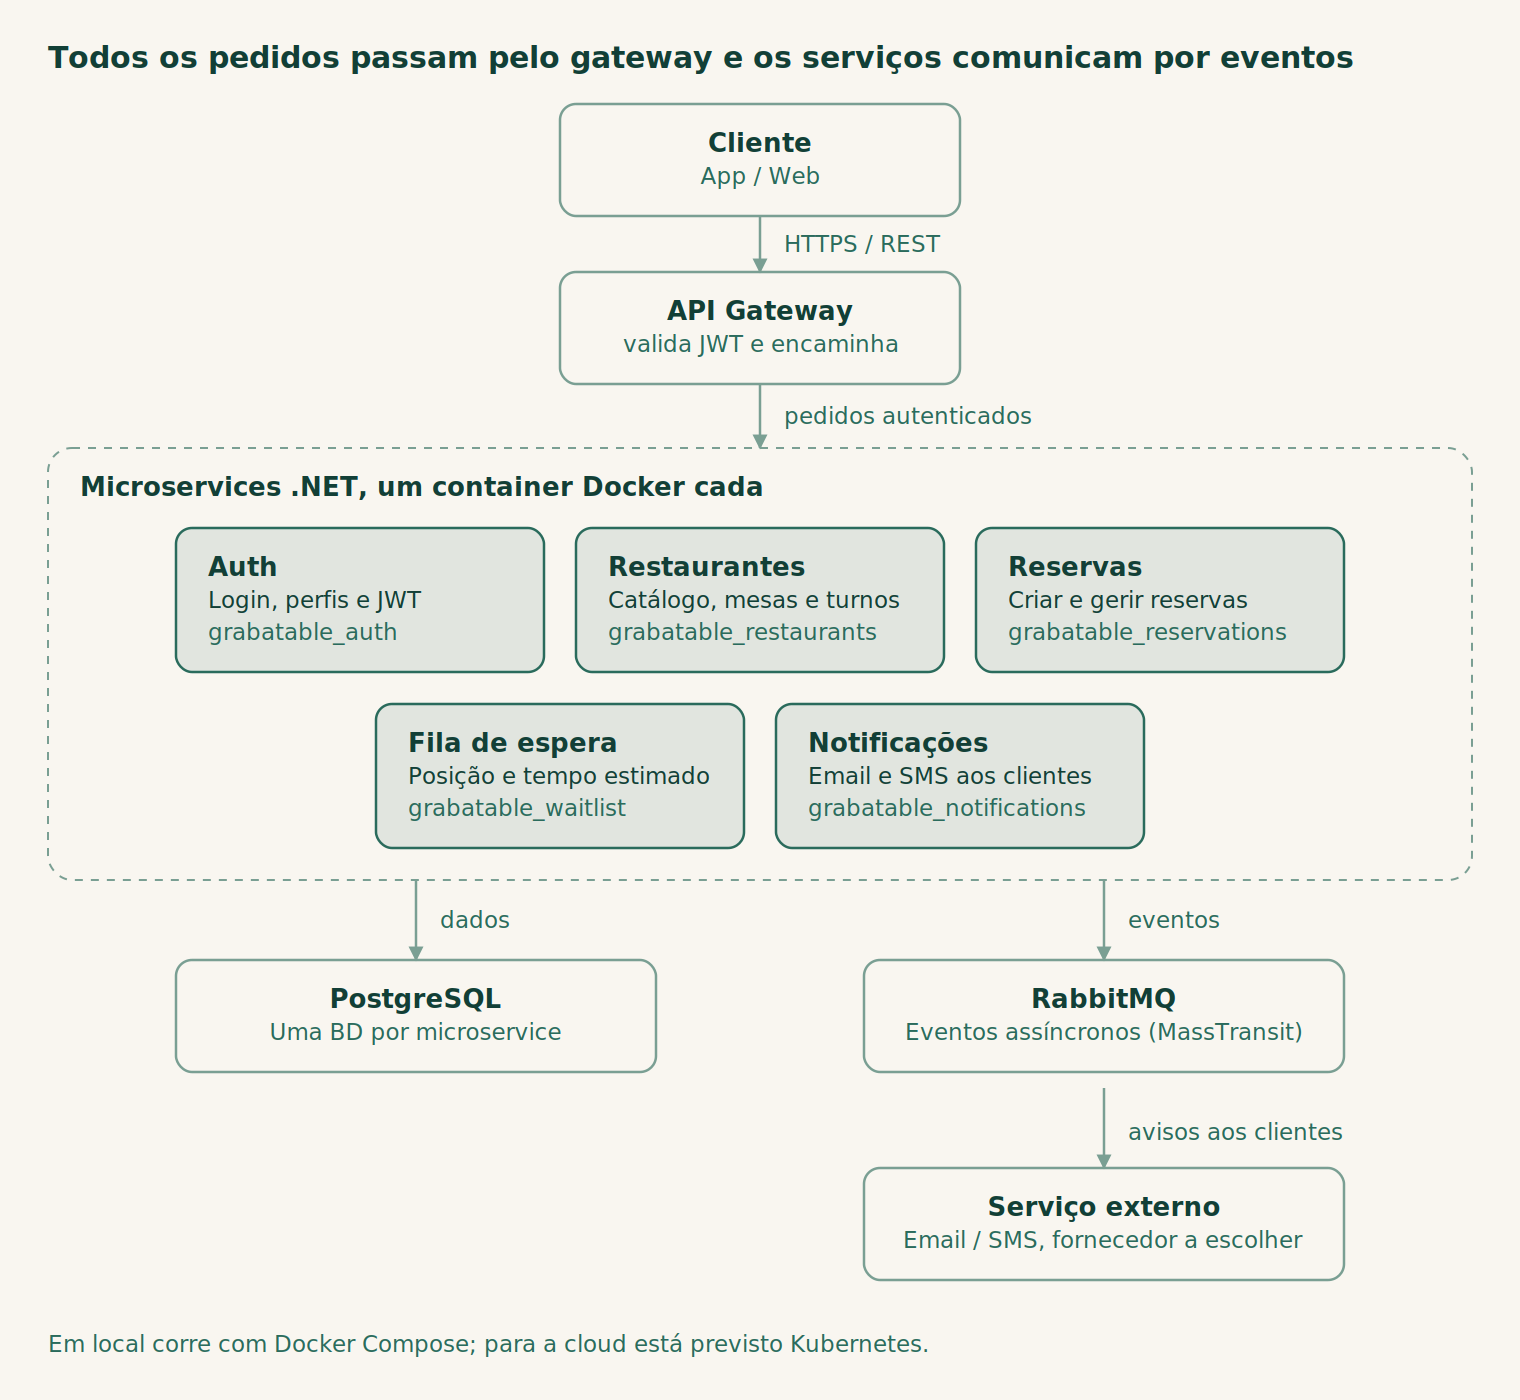
\includegraphics[width=1.0\linewidth]{images/arquitetura.png}
    \caption{Arquitetura Técnica do Sistema}
    \label{fig:10}
\end{figure}

O \textit{gateway} é o único ponto exposto: valida o \textit{JWT} e encaminha cada pedido para o microsserviço certo. Cada serviço tem a sua base de dados no mesmo PostgreSQL. Reservas e Fila de espera publicam eventos no \textit{RabbitMQ}~\cite{rabbitmq}, e o serviço de Notificações consome-os para avisar o cliente.

\section{BPMN}

O diagrama BPMN representa o fluxo dos principais processos do sistema GrabATable, permitindo visualizar de forma estruturada as atividades realizadas pelos diferentes intervenientes. Através deste modelo, é possível compreender a sequência das tarefas, as decisões e interações entre os diferentes participantes, proporcionando uma visão global do funcionamento dos processos da plataforma.

\begin{figure}[H]
    \centering
    
\includegraphics[width=1.0\linewidth]{images/BPMN.png}
    \caption{Diagrama BPMN}
    \label{fig:11}
\end{figure}

\section{Personas}
 
As \textit{personas} são perfis fictícios, construídos a partir dos três perfis de utilizador definidos na Secção 1.2, que representam os objetivos, o contexto de uso e as frustrações dos utilizadores reais da plataforma.
 
\subsection{Persona 1 -- Marta Silva (Cliente)}
 
\begin{tabularx}{\textwidth}{@{}>{\bfseries}p{3.4cm}X@{}}
\toprule
Perfil & Cliente \\
Idade e profissão & 34 anos, designer gráfica \\
Localização & Braga \\
Competência digital & Alta; usa o telemóvel para quase tudo, incluindo pagamentos e marcações \\
Contexto de uso & Telemóvel, em casa ou no trabalho, a organizar jantares com antecedência \\
\midrule
Objetivos &
\begin{itemize}[nosep,leftmargin=*]
  \item Reservar mesa para um grupo de 4 a 6 pessoas, sem telefonar;
  \item Ter confirmação imediata e poder alterar ou cancelar a reserva;
  \item Receber um lembrete antes da data.
\end{itemize} \\
Frustrações &
\begin{itemize}[nosep,leftmargin=*]
  \item Restaurantes que só aceitam reservas por telefone, em horário de expediente;
  \item Chegar à hora marcada e esperar por uma mesa que devia estar livre;
  \item Não saber se a reserva ficou realmente registada.
\end{itemize} \\
Cenário &
A Marta quer jantar com amigos na sexta-feira. Pesquisa restaurantes por cozinha e hora, confirma a disponibilidade para seis pessoas, reserva em poucos toques e recebe a notificação de confirmação. \\
Requisitos associados & RF03, RF04, RF05, RF06, RF08 \\
\bottomrule
\end{tabularx}
 
\subsection{Persona 2 -- Rui Fernandes (Cliente sem reserva)}
 
\begin{tabularx}{\textwidth}{@{}>{\bfseries}p{3.4cm}X@{}}
\toprule
Perfil & Cliente \\
Idade e profissão & 27 anos, técnico de logística \\
Localização & Guimarães \\
Competência digital & Média-alta; usa aplicações móveis no dia a dia, mas pouco paciente com processos longos \\
Contexto de uso & Telemóvel, muitas vezes a caminho do restaurante, com pouco tempo e uma só mão livre \\
\midrule
Objetivos &
\begin{itemize}[nosep,leftmargin=*]
  \item Entrar na fila antes de chegar ao restaurante;
  \item Saber a posição e o tempo estimado de espera;
  \item Ser avisado quando a mesa estiver quase pronta, para poder fazer outra coisa entretanto.
\end{itemize} \\
Frustrações &
\begin{itemize}[nosep,leftmargin=*]
  \item Esperas de pé, sem qualquer estimativa;
  \item Estimativas dadas ao balcão que nunca se cumprem;
  \item Perder a vez por ter saído para ir buscar o carro.
\end{itemize} \\
Cenário &
O Rui decide jantar fora de improviso. Abre a aplicação, escolhe um restaurante, entra na fila para duas pessoas e vê que a espera é de cerca de 25 minutos. Recebe um aviso quando a mesa está próxima de ficar disponível. \\
Requisitos associados & RF03, RF04, RF07, RF08 \\
\bottomrule
\end{tabularx}
 
\subsection{Persona 3 -- Teresa Almeida (Gestora)}
 
\begin{tabularx}{\textwidth}{@{}>{\bfseries}p{3.4cm}X@{}}
\toprule
Perfil & Gestor \\
Idade e profissão & 45 anos, responsável de sala num restaurante com 18 mesas \\
Localização & Porto \\
Competência digital & Média; usa tablet e computador, mas valoriza ferramentas simples \\
Contexto de uso & Tablet à entrada da sala, durante o serviço, sob pressão de tempo e com interrupções constantes \\
\midrule
Objetivos &
\begin{itemize}[nosep,leftmargin=*]
  \item Ver num só ecrã a ocupação das mesas, as reservas do dia e a fila;
  \item Registar chegadas, sentar clientes e libertar mesas com poucos toques;
  \item Reduzir as faltas de comparação e a sobrelotação.
\end{itemize} \\
Frustrações &
\begin{itemize}[nosep,leftmargin=*]
  \item Caderno de reservas em papel e lista de espera improvisada;
  \item Mesas reservadas que ficam vazias por não comparência;
  \item Clientes sem reserva que se queixam de esperas sem explicação.
\end{itemize} \\
Cenário &
Em plena hora de ponta, a Teresa regista a chegada de um grupo com reserva, vê que há uma mesa a libertar-se e chama o próximo grupo da fila, sem sair do tablet. \\
Requisitos associados & RF09, RF10, RF11, RF12 \\
\bottomrule
\end{tabularx}
 
\subsection{Persona 4 -- Pedro Machado (Administrador)}
 
\begin{tabularx}{\textwidth}{@{}>{\bfseries}p{3.4cm}X@{}}
\toprule
Perfil & Administrador \\
Idade e profissão & 38 anos, membro da equipa responsável pela plataforma \\
Localização & Remoto \\
Competência digital & Muito alta; confortável com painéis de administração e relatórios \\
Contexto de uso & Computador, de forma pontual, para configurar e supervisionar \\
\midrule
Objetivos &
\begin{itemize}[nosep,leftmargin=*]
  \item Adicionar e configurar novos restaurantes e respetivas contas de gestor;
  \item Definir políticas globais (regras de não comparência, tempo médio de refeição);
  \item Consultar relatórios por restaurante e por região.
\end{itemize} \\
Frustrações &
\begin{itemize}[nosep,leftmargin=*]
  \item Configurações dispersas por vários ecrãs;
  \item Falta de histórico sobre quem alterou o quê;
  \item Dificuldade em identificar clientes com faltas repetidas.
\end{itemize} \\
Cenário &
O Pedro integra um novo restaurante: cria o registo, cria a conta do gestor e confirma a configuração, tudo a partir da Gestão de restaurantes. \\
Requisitos associados & RF13, RF14, RF15, RF16 \\
\bottomrule
\end{tabularx}
 
 
% ============================================================
 
\section{Análise SWOT}
 
A análise SWOT identifica os fatores internos (forças e fraquezas) e externos (oportunidades e ameaças) que podem influenciar o sucesso do GrabATable. Serve para orientar prioridades de desenvolvimento e antecipar riscos.
 
\begin{table}[ht]
\centering
\small
\renewcommand{\arraystretch}{1.25}
\begin{tabularx}{\textwidth}{@{}>{\raggedright\arraybackslash}X>{\raggedright\arraybackslash}X@{}}
\toprule
\textbf{Forças (interno)} & \textbf{Fraquezas (interno)} \\
\midrule
\begin{itemize}[nosep,leftmargin=*]
  \item Fila de espera gerida em conjunto com as reservas, e não como lista à parte;
  \item Estimativa de espera dinâmica, calculada com reservas, tempo médio de refeição e fila ativa;
  \item Arquitetura de microsserviços, resiliente e escalável (RNF04, RNF05);
  \item Sistema visual com acessibilidade cromática verificada (WCAG 2.1 AA).
\end{itemize}
&
\begin{itemize}[nosep,leftmargin=*]
  \item A qualidade da estimativa depende de dados que o gestor tem de registar (chegadas, mesas libertadas);
  \item Tempo médio de refeição é uma média, que pode falhar em casos atípicos;
\end{itemize} \\
\midrule
\textbf{Oportunidades (externo)} & \textbf{Ameaças (externo)} \\
\midrule
\begin{itemize}[nosep,leftmargin=*]
  \item Muitos restaurantes ainda gerem reservas em papel ou por telefone;
  \item Elevada utilização do telemóvel e habituação a serviços de marcação digitais;
  \item Valor acrescentado das estatísticas de ocupação e não comparência para os restaurantes;
  \item Possibilidade de integração futura com sistemas de ponto de venda;
  \item Expansão para outras regiões, aproveitando a escalabilidade horizontal.
\end{itemize}
&
\begin{itemize}[nosep,leftmargin=*]
  \item Plataformas de reservas já estabelecidas, com muitos restaurantes e utilizadores;
  \item Resistência dos gestores a mudar processos durante o serviço;
  \item Cumprimento do RGPD e riscos associados a dados pessoais (RNF09);
  \item Dependência de serviços externos de notificação e respetivos custos;
  \item Não comparência e abuso da fila, que podem prejudicar a confiança no sistema.
\end{itemize} \\
\bottomrule
\end{tabularx}
\caption{Análise SWOT do GrabATable}
\end{table}